\section{Printed Room Labels}
\label{sec:ocr}

Every experiment so far left rare-class AP at or near zero, and the frozen
DINOv2 classifier failed on rare rooms even when handed ground-truth crops.
Looking at the plans suggests why. Rooms of different classes often share
geometry and furniture symbols, and what separates them is the name printed
inside. In Figure~\ref{fig:predmulticlass} a room printed ``Spindraum'' is a
Garderobe, and a room printed ``Aufenthalt'' is a Versammlungsraum. The
detector sees each plan at no more than 1600 pixels per side, where those names
are a few pixels high, and none of the augmentation strategies changed the
printed name to match the new class. Goal 6 therefore treats the printed label
as an input. Section~\ref{sec:ocrmethod} describes the implementation.

The work ran in two stages. A pre-registered study
(\code{docs/preregistration_ocr.md}, Section~\ref{sec:ocrstudy}) tested the text
branch and label replacement with 12 seeds per arm. A follow-up designed after
its results (\code{docs/preregistration_followup.md},
Section~\ref{sec:followup}) is exploratory by construction. Both use the
multiclass track, seeds 1001 to 1012, the unchanged training recipe, and mask
AP of \code{last.pth} on the 21 held-out plans. The control e0 is the set of 12
multiclass runs of Section~\ref{sec:confirmmc}, reused without retraining.

\subsection{How much class information the labels carry}

OCR finds at least one label token in 87\,\% of the held-out rooms and in 39 of
the 40 held-out rare rooms. In the training plans the figure is 52\,\%, because
several training projects print only room numbers. Table~\ref{tab:ocrstage1}
classifies the 746 ground-truth rooms of the 21 held-out plans from their tokens
alone, which removes detector error. The classifiers were trained on the
training rooms with fixed hyperparameters and nothing was tuned on held-out
plans.

\begin{table}[H]
\centering
\caption{Classification of the 746 ground-truth rooms of the 21 held-out plans.
Zero-shot assigns the class whose name is most similar to the room's tokens;
the other heads are logistic regressions on the training rooms. The visual
head uses the frozen DINOv2 crop features of Section~\ref{sec:results}. The
last row adds the 412 rare rooms converted by copy-paste for e24
(Section~\ref{sec:followup}) to the training rooms of the text head.}
\label{tab:ocrstage1}
\small
\begin{tabular}{@{}lrrrr@{}}
\toprule
Head & Top-1 & Macro recall & Recall, frequent & Recall, rare \\
\midrule
Zero-shot class-name similarity & 0.674 & 0.452 & 0.625 & 0.315 \\
Text features & 0.601 & 0.393 & 0.620 & 0.144 \\
DINOv2 visual features & 0.452 & 0.218 & 0.392 & 0.000 \\
Text and visual features & 0.729 & 0.433 & 0.712 & 0.111 \\
\midrule
Text features, with synthetic rare rooms & 0.678 & 0.430 & 0.624 & 0.249 \\
\bottomrule
\end{tabular}
\end{table}

Text lifts top-1 accuracy from 0.452 to 0.729 when added to the visual
features, and every head that reads text recalls some rare rooms where the
visual head recalls none. The visual head scores 0.452 here, against 0.454 in
Table~\ref{tab:dino}, because it is evaluated on the rooms of all 21 held-out
plans instead of the 368 test rooms. The zero-shot rule, which uses no training rooms,
has the best rare recall. The learned heads see only 30 rare training rooms,
many of them without a readable name, and they fit the vocabulary of the
training projects. A ``Spindraum'' in a held-out building has no counterpart in
training, while its embedding still lies closer to Garderobe than to most other
class names.

The same text classifier can label the masks of a class-agnostic detector. With
the masks of the 12 class-agnostic e0 runs, this two-stage system reaches
$0.213$ multiclass mask AP against $0.100$ for the multiclass e0 runs. It is
higher on every one of the 12 seeds (range $0.197$ to $0.225$, against at most
$0.106$ for e0), and its rare-class AP is $0.099$ where e0 scores zero. This
comparison was specified as descriptive in the pre-registration, so it carries
no formal test, but it shows that the text holds class information which the
end-to-end detector does not use.

\subsection{Pre-registered study}
\label{sec:ocrstudy}

The study tested three hypotheses, each one-sided and paired over seeds (arms
with the same seed share the per-epoch plan order): H6, the text branch
improves on the plain model (e19 against e0); H7, label replacement adds to the
text branch (e20 against e19); H8, label replacement helps the plain model (e18
against e0). Holm's correction runs over the three, and a hypothesis counts as
supported only if Holm rejects and the paired seed $\times$ image bootstrap
95\,\% CI excludes zero. The smallest effect of interest is $+0.01$ AP.
Amendment 1, recorded before any detector run, changed how the vocabulary of
rendered names is built after a dry run on six rooms showed OCR fragments such
as ``raum'' in it.

\paragraph{Label replacement yield.} Of 104 planned room edits, 32 were
rejected because the rare-class name did not fit inside the room, 20 because
the erasure failed its check and 4 because the room interior was empty after
erosion; 2 raised errors. Of the 46 generated rooms, the diffusion fill passed
the erasure check in 5 and Telea inpainting erased the label in 29; the other
12 had no OCR label to erase and only received the new name. OCR then read the new name
and no longer the old one in 34 of the 46 generated rooms. The admitted rooms
form 23 synthetic variants of 12 training plans and convert 34 rooms, 17 of
them to Versammlungsraum and none to Garderobe. Each run of e18 or e20 saw
about 226 converted rooms. Figure~\ref{fig:labelreplacement} shows admitted
examples.

\begin{figure}[H]
\centering
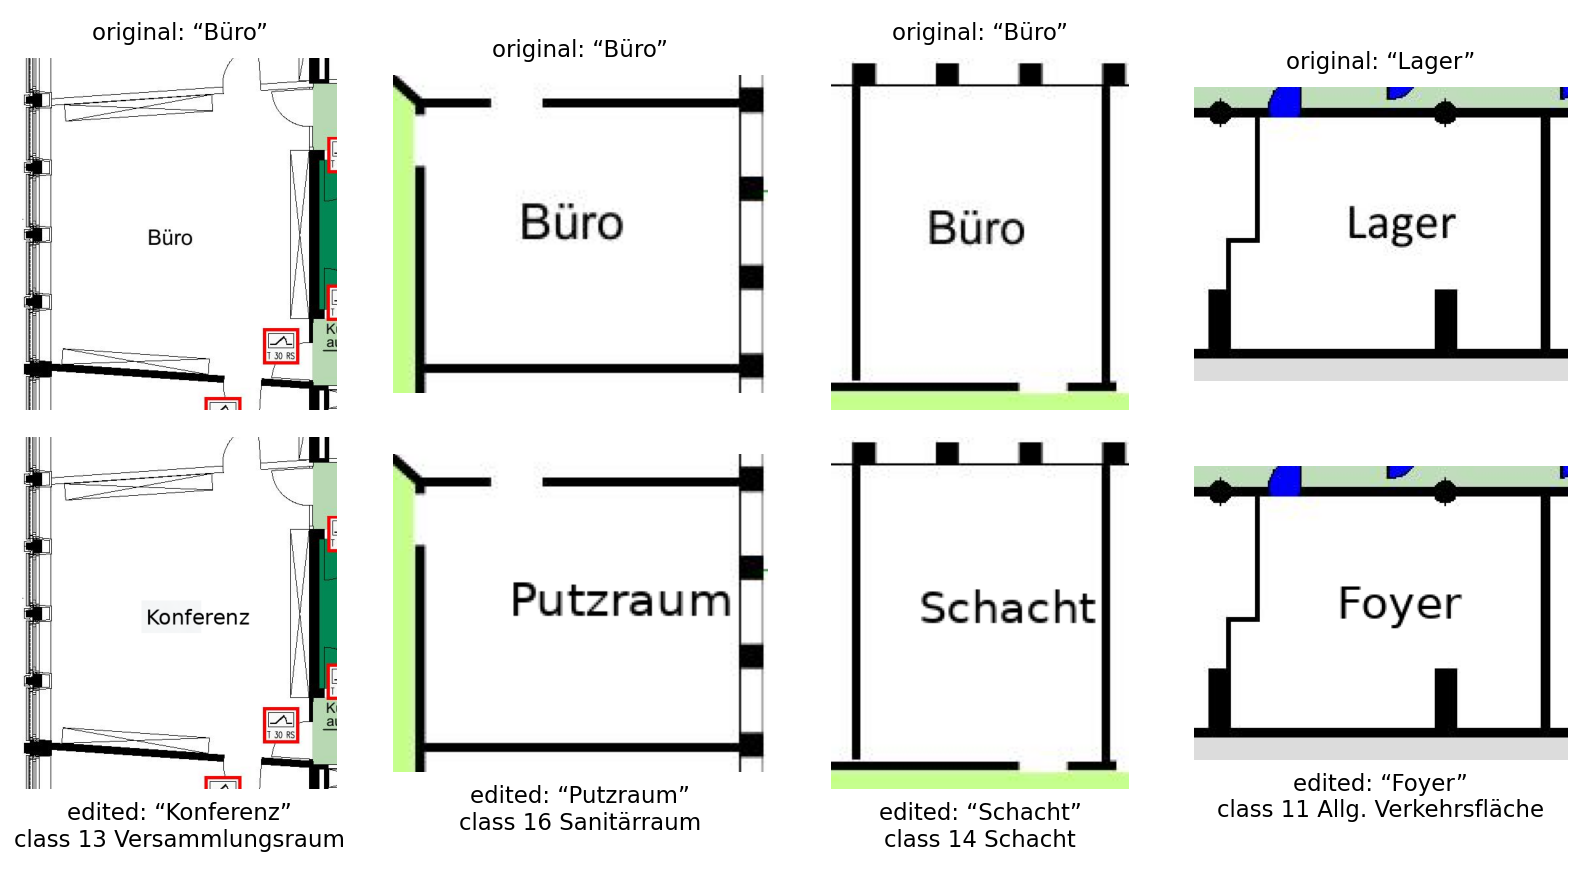
\includegraphics[width=\textwidth]{images/fig_label_replacement.png}
\caption{Admitted label replacements. Top: training rooms with their original
name. Bottom: the name erased and a rare-class name rendered in its place; the
annotation carries the new class. The first column was erased by diffusion,
the others by Telea inpainting.}
\label{fig:labelreplacement}
\end{figure}

\begin{table}[H]
\centering
\caption{Pre-registered OCR study: multiclass mask AP of \code{last.pth}, mean
$\pm$ s.d.\ over 12 seeds.}
\label{tab:ocrarms}
\small
\begin{tabular}{@{}llrrrr@{}}
\toprule
Arm & Method & AP (21) & AP50 (21) & AP (11 test) & Rare AP \\
\midrule
e0 & Plain model & 0.100 $\pm$ 0.006 & 0.146 $\pm$ 0.007 & 0.090 $\pm$ 0.005 & 0.000 \\
e18 & Plain model, replaced labels & 0.099 $\pm$ 0.006 & 0.143 $\pm$ 0.006 & 0.088 $\pm$ 0.010 & 0.000 \\
e19 & Text branch & 0.093 $\pm$ 0.006 & 0.137 $\pm$ 0.007 & 0.083 $\pm$ 0.008 & 0.000 \\
e20 & Text branch, replaced labels & 0.096 $\pm$ 0.007 & 0.140 $\pm$ 0.010 & 0.086 $\pm$ 0.008 & 0.000 \\
\bottomrule
\end{tabular}
\end{table}

\begin{table}[H]
\centering
\caption{Pre-registered contrasts. $\Delta$ is treatment minus control; the CI
resamples seed pairs and the 21 held-out plans, the second CI resamples
projects before plans; $p$ is the one-sided paired $t$-test.}
\label{tab:ocrtests}
\small
\begin{tabular}{@{}lrrrrrl@{}}
\toprule
Contrast & $\Delta$ & 95\% CI & CI by project & $p$ & Holm $p$ & Supported \\
\midrule
H6: e19 $-$ e0 & $-0.006$ & [$-0.012$, $+0.000$] & [$-0.015$, $+0.005$] & 1.000 & 1.000 & no \\
H7: e20 $-$ e19 & $+0.002$ & [$-0.004$, $+0.008$] & [$-0.006$, $+0.008$] & 0.142 & 0.425 & no \\
H8: e18 $-$ e0 & $-0.001$ & [$-0.006$, $+0.003$] & [$-0.008$, $+0.006$] & 0.778 & 1.000 & no \\
\bottomrule
\end{tabular}
\end{table}

No hypothesis is supported, and for all three the upper bound of the CI lies
below the smallest effect of interest. Rare-class AP is zero in every run.
After training, the weights explain the result for the text branch. The norm of
its last layer reached 0.24, against 3.1 for the classification layer it feeds,
and its first layer barely changed. A branch that starts at
zero receives small gradients, and under the detector's schedule the learning
rate falls tenfold after 280 of the 875 steps, so the branch never contributed.
This diagnosis came after the results and was tested in the follow-up. Label
replacement had a different problem: 226 converted rooms per run, read by a
model that cannot resolve the text, change nothing measurable.

\subsection{Follow-up experiments}
\label{sec:followup}

The follow-up asked four questions raised by the study: whether the text branch
helps once it can train (e21), whether copy-paste helps when it brings the rare
classes close to balance (e22 to e24), whether the two-stage text classifier
gains from synthetic rare rooms, and how the text classifier performs on SAM 3
masks. The contrasts for e21 and e22 to e24 follow the same paired tests and
CI rule as the study, with Holm's correction within each group. The dose trend
is a one-sided test of the per-seed regression slope of AP on the number of
converted rooms. All results here are exploratory.

\begin{table}[H]
\centering
\caption{Follow-up arms: multiclass mask AP of \code{last.pth} on the 21
held-out plans, mean $\pm$ s.d.\ over 12 seeds. Converted rooms are the rare
rooms added by copy-paste.}
\label{tab:followuparms}
\small
\begin{tabular}{@{}llrrrr@{}}
\toprule
Arm & Method & Converted & AP (21) & AP50 (21) & Rare AP \\
\midrule
e0 & Plain model & 0 & 0.100 $\pm$ 0.006 & 0.146 $\pm$ 0.007 & 0.000 $\pm$ 0.000 \\
e19 & Text branch (study) & -- & 0.093 $\pm$ 0.006 & 0.137 $\pm$ 0.007 & 0.000 $\pm$ 0.000 \\
e21 & Text branch, own AdamW & -- & 0.184 $\pm$ 0.018 & 0.265 $\pm$ 0.026 & 0.015 $\pm$ 0.026 \\
e22 & Copy-paste, 20 per rare class & 69 & 0.094 $\pm$ 0.005 & 0.139 $\pm$ 0.006 & 0.002 $\pm$ 0.003 \\
e23 & Copy-paste, 50 per rare class & 205 & 0.087 $\pm$ 0.007 & 0.127 $\pm$ 0.009 & 0.003 $\pm$ 0.002 \\
e24 & Copy-paste, 100 per rare class & 412 & 0.082 $\pm$ 0.006 & 0.120 $\pm$ 0.008 & 0.005 $\pm$ 0.003 \\
\bottomrule
\end{tabular}
\end{table}

\begin{table}[H]
\centering
\caption{Follow-up contrasts (exploratory). CIs and $p$ as in
Table~\ref{tab:ocrtests}; Holm runs within the copy-paste group and within the
text branch group.}
\label{tab:followuptests}
\small
\begin{tabular}{@{}lrrrrl@{}}
\toprule
Contrast & $\Delta$ & 95\% CI & CI by project & Holm $p$ & Supported \\
\midrule
e21 $-$ e0 & $+0.085$ & [$+0.070$, $+0.112$] & [$+0.061$, $+0.131$] & $<0.001$ & yes \\
e21 $-$ e19 & $+0.091$ & [$+0.077$, $+0.119$] & [$+0.062$, $+0.141$] & $<0.001$ & yes \\
e22 $-$ e0 & $-0.005$ & [$-0.012$, $+0.001$] & [$-0.014$, $+0.001$] & 1.000 & no \\
e23 $-$ e0 & $-0.013$ & [$-0.020$, $-0.006$] & [$-0.024$, $-0.004$] & 1.000 & no \\
e24 $-$ e0 & $-0.017$ & [$-0.027$, $-0.009$] & [$-0.032$, $-0.006$] & 1.000 & no \\
\bottomrule
\end{tabular}
\end{table}

\begin{figure}[H]
\centering
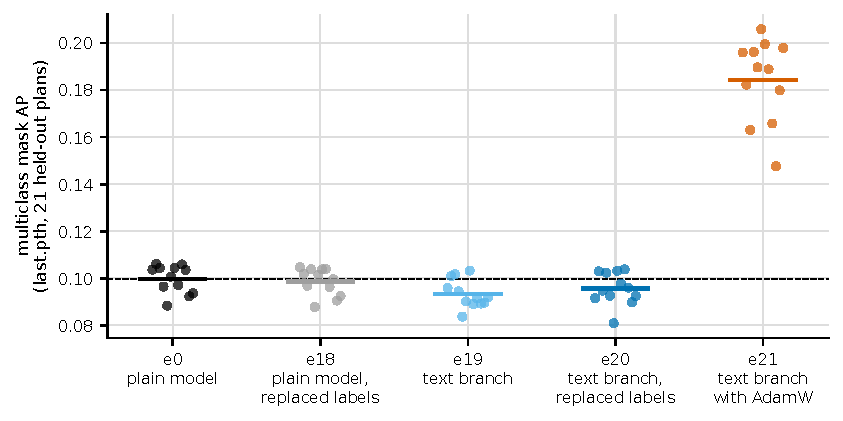
\includegraphics[width=0.9\textwidth]{images/fig_text_runs.pdf}
\caption{Multiclass mask AP per seed for the plain model, the text branch arms
and the label replacement arms. Bars mark the mean; the dashed line is the mean
of e0.}
\label{fig:textruns}
\end{figure}

\paragraph{A text branch that trains.} With its own optimiser and pooling
restricted to tokens inside the proposal, the text branch almost doubles
multiclass mask AP, from $0.100$ to $0.184$. The lowest of the 12 e21 seeds
($0.148$) lies above the highest e0 seed ($0.106$), and the interval stays
above zero when whole projects are resampled. Figure~\ref{fig:textperclass}
shows where the gain comes from. Classes with distinctive names gain most:
K\"uche rises from $0.040$ to $0.423$, Besprechungsraum from $0.042$ to $0.506$,
Lager from $0.120$ to $0.393$ and B\"uroraum from $0.543$ to $0.754$. Classes
that the plan identifies by symbols, such as Treppe and Aufzug, change little.
Rare-class AP rises only to $0.015$, with a standard deviation larger than its
mean: one rare class, Abstellraum, reaches $0.085$, and the others stay near
zero. The seed spread of e21 is three times that of e0, so the branch trains,
but not equally well in every run.

\begin{figure}[H]
\centering
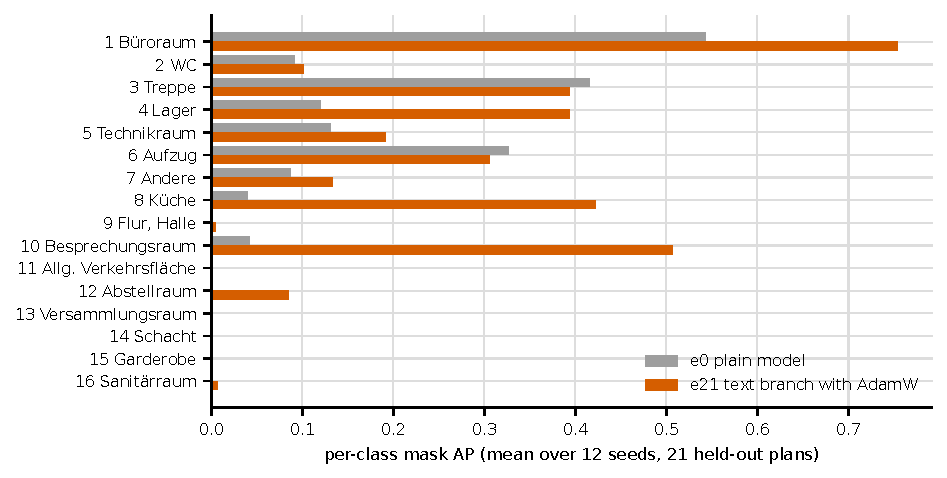
\includegraphics[width=0.9\textwidth]{images/fig_text_perclass.pdf}
\caption{Per-class mask AP of the plain model (e0) and the text branch with its
own optimiser (e21), mean over 12 seeds on the 21 held-out plans.}
\label{fig:textperclass}
\end{figure}

\paragraph{Copy-paste towards class balance.} The three copy-paste doses
reached 69, 205 and 412 converted rooms. For the largest dose this brings every
rare class to between 63 and 95 training instances, against 3 to 8 real ones;
classes with only three real donor rooms are limited by the reuse cap. Overall
AP falls with every step in dose (Figure~\ref{fig:dose}), with a mean slope of
$-0.004$ AP per 100 converted rooms, and the losses at 205 and 412 rooms have
intervals below zero. Rare-class AP rises from zero to $0.005$, too little to
offset the losses on frequent classes. K\"uche falls from $0.040$ to $0.009$
and WC from $0.091$ to $0.033$, while Besprechungsraum drops to zero. The
pasted rooms repeat the same 30 real rare rooms many times, and each conversion
removes a frequent room with its original label from the synthetic plan, so the
model sees more copies of a few rare appearances and fewer correct frequent
examples.

\begin{figure}[H]
\centering
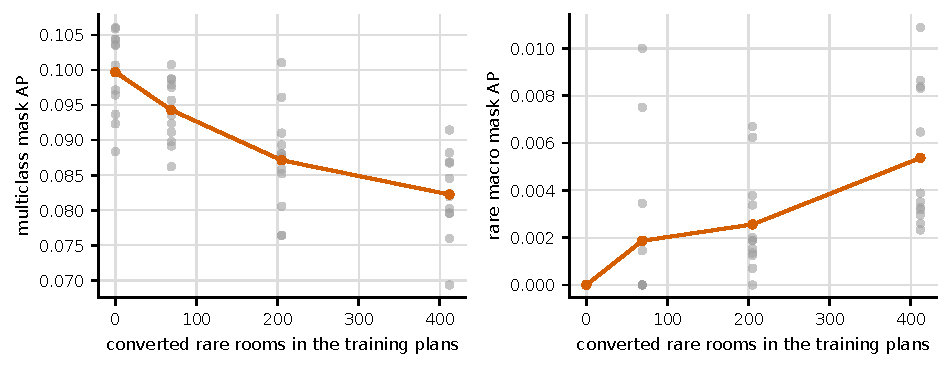
\includegraphics[width=\textwidth]{images/fig_dose_response.pdf}
\caption{Copy-paste dose against multiclass mask AP (left) and rare-class macro
AP (right). Grey dots are seeds, the line connects the means of e0, e22, e23
and e24.}
\label{fig:dose}
\end{figure}

\paragraph{Two-stage text classification.} Adding the 412 converted rare rooms
of e24, read by the same OCR, to the training rooms of the two-stage text
classifier raises its multiclass AP from $0.213$ to $0.221$ and its rare-class
AP from $0.099$ to $0.126$, on the same 12 sets of class-agnostic masks
(paired $p < 0.001$ for both). On the ground-truth rooms of
Table~\ref{tab:ocrstage1} the same addition raises the top-1 accuracy of the
text head from $0.601$ to $0.678$ and its rare recall from $0.144$ to $0.249$.
Synthetic rare rooms help the classifier that reads text, where they hurt the
detector.

\paragraph{SAM 3 masks.} The classifier trained with the synthetic rare rooms,
labelling the class-agnostic SAM 3 masks on the 11 test plans, reaches $0.258$ multiclass mask AP and $0.084$ rare
AP, against $0.115$ and zero for the fine-tuned multiclass SAM 3
(Table~\ref{tab:ocrsam3}). This is the highest multiclass score in the project,
from a single SAM 3 run, and it is descriptive.

\begin{table}[H]
\centering
\caption{Multiclass mask AP on the 11 test plans. The two-stage row labels
class-agnostic SAM 3 masks with the OCR text classifier trained on the real and
the 412 synthetic rare rooms; the Mask R-CNN row is a mean over 12 seeds, the
SAM 3 rows are single runs.}
\label{tab:ocrsam3}
\small
\begin{tabular}{@{}lrrr@{}}
\toprule
Method & Mask AP & AP50 & Rare AP \\
\midrule
Mask R-CNN e0, multiclass & 0.090 & -- & 0.000 \\
SAM 3, multiclass & 0.115 & 0.152 & 0.000 \\
SAM 3 class-agnostic masks + OCR text classifier & 0.258 & 0.335 & 0.084 \\
\bottomrule
\end{tabular}
\end{table}

\subsection{Interpretation}

The printed room name is the strongest class cue in this dataset, and a model
that reads it improves multiclass segmentation by a margin larger than any
other change in the project. Synthetic rooms do not substitute for it. Label
replacement could not be tested at a useful dose, because most rare-class names
do not fit inside the frequent rooms they would replace, and copy-paste towards
balance reduced AP as the dose grew. Synthetic rare rooms helped only the
classifier that reads text. A pasted room carries the printed name of its real
donor, so it repeats a rare name and raises the weight of its class, while the
detector receives only more copies of a few rare appearances. The best system
of the project, the text classifier on SAM 3 masks, was trained with these
rooms. Their contribution was measured on the Mask R-CNN masks only, so the
SAM 3 figure is not a measured gain from synthetic data.

The follow-up was designed after the study's results, so its findings are hypotheses for a further confirmation, not confirmed effects.
The 21 held-out plans come from three buildings and have been used to evaluate
earlier arms. Rare-class AP stays low even for the best systems, between
$0.015$ for e21 and $0.126$ for the two-stage classifier, because many rare
rooms carry names that do not occur in the training plans.
